\documentclass[pdf,9pt,aspectratio=169]{beamer}
\usepackage[utf8]{inputenc}

\usepackage{DejaVuSans}
\usepackage{DejaVuSerif}
\usepackage{DejaVuSansMono}
\usepackage[T2A]{fontenc}

\usepackage[russian]{babel}

\usepackage{hyperref}
\hypersetup{unicode=true}

\usetheme{Madrid}
\usefonttheme[stillsansserifsmall]{serif}
%\usefonttheme[onlylarge]{structurebold}
\usefonttheme[onlylarge]{structureitalicserif}

\title[]{Архитектура компьютера}
\subtitle{Введение в предмет}
\author[]{Александр Рудалёв}
\institute[]{ИМИКТ САФУ}
\date[]{2016}

\usepackage{wrapfig}
\usepackage{color}
\usepackage{xcolor}

\usepackage{tikz}
\usetikzlibrary{arrows}
\usetikzlibrary{babel}
\usetikzlibrary{shapes}
\usetikzlibrary{positioning}

\tikzset{
  MyChar/.style={
    rectangle, rounded corners=1mm,
    minimum height=6mm,
    minimum width=4.8mm,
    very thick, draw=black!50,
    top color=white,bottom color=black!20,
  },
}

\usepackage{minted}
\usemintedstyle{default} 
\newcommand{\cpil}[1]{\mintinline{python3}{#1}}

\begin{document}

\frame{\titlepage}

%%%%%%%%%%%%%%%%%%%%%%%%%%%%%%%%%%%%%%%%%%%%%%%%%%%%%%%%%%%%%%%%%%%%%%%%%%%%%%%
%%
%% Определения
%%
\begin{frame}\frametitle{Введение в предмет <<Архитектура компьютера>>}
  \begin{block}<1->{Определение}
    \textbf{Архитектура компьютера} "---  это описание его организации и принципов функционирования его структурных элементов. Включает основные устройства ЭВМ и структуру связей между ними.
  \end{block}
  \begin{block}<2->{О чём пойдёт речь}
    В рамках дисциплины мы должны понять как работает компьютер и программное обеспечение на нём.
  \end{block}
\end{frame}

%%%%%%%%%%%%%%%%%%%%%%%%%%%%%%%%%%%%%%%%%%%%%%%%%%%%%%%%%%%%%%%%%%%%%%%%%%%%%%%
%%
%% Вопрос
%%
\begin{frame}{Вопрос}
  \begin{columns}[c]
    \begin{column}[]{0.5\textwidth}  
      \begin{alertblock}<1->{Что это?}
        \begin{figure}
          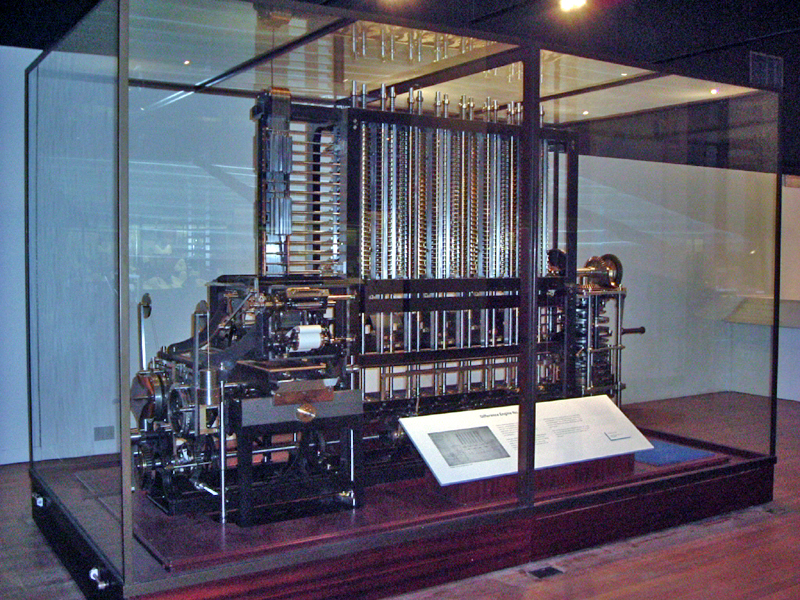
\includegraphics[width=\textwidth]{images/DifferenceEngine.jpg}
        \end{figure}
      \end{alertblock}
    \end{column}
  \end{columns}
\end{frame}

%%%%%%%%%%%%%%%%%%%%%%%%%%%%%%%%%%%%%%%%%%%%%%%%%%%%%%%%%%%%%%%%%%%%%%%%%%%%%%%
%%
%% Вопрос
%%
\begin{frame}{Вопрос}
  \begin{columns}[c]
    \begin{column}[]{0.35\textwidth}  
      \begin{alertblock}<1->{Что это?}
        \begin{figure}
          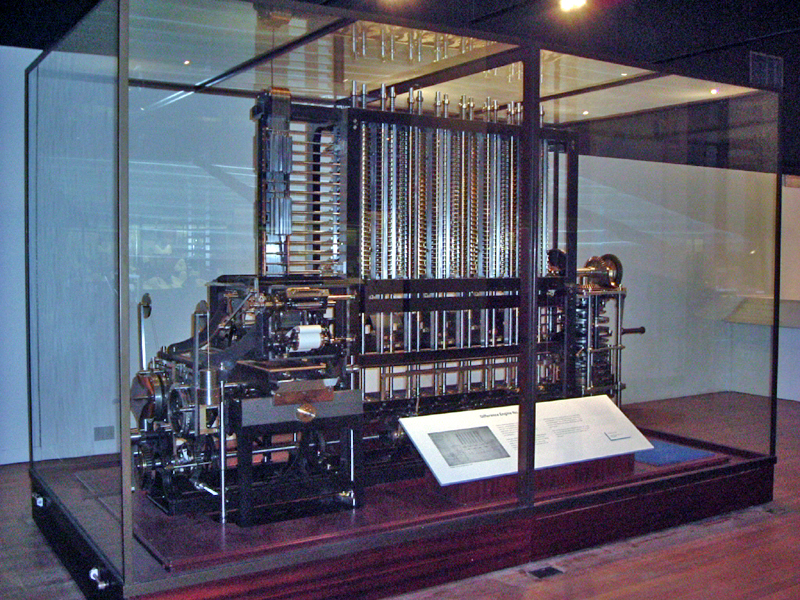
\includegraphics[width=\textwidth]{images/DifferenceEngine.jpg}
        \end{figure}
      \end{alertblock}
    \end{column}
    \begin{column}[]{0.55\textwidth}
      \begin{exampleblock}<1->{Разностная машина Чарльза Бэббиджа}
        \begin{columns}[]
          \column{2cm}
            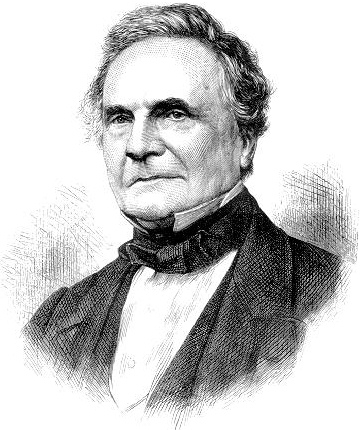
\includegraphics[width=\textwidth]{images/CharlesBabbage.jpg}
          \column{5.7cm}
              \setlength{\leftmargini}{5pt}
            \begin{itemize}
              \item До: Суммирующая машина Паскаля (1642 г.).
              \item Применение: Вычисление логарифмических таблиц.
              \item Первая статья: 1822 г.
              \item Реализация работающей копии: 1989-1991 гг.
            \end{itemize}
        \end{columns}
        \begin{itemize}
          \item Прообраз для: Аналитической машины.
          \item На её основе в 1854 г. Георг Шутц строит более простую <<машину вычислений>>.
          \item Р.С.~Гутер, Ю.Л.~Полунов <<От абака до компьютера>>
        \end{itemize}
      \end{exampleblock}
    \end{column}
  \end{columns}
\end{frame}


%%%%%%%%%%%%%%%%%%%%%%%%%%%%%%%%%%%%%%%%%%%%%%%%%%%%%%%%%%%%%%%%%%%%%%%%%%%%%%%
%%
%% 
%%
\begin{frame}{Аналитическая машина Чарльза Бэббиджа}
  \begin{columns}[T]
    \begin{column}[]{0.45\textwidth}  
      \begin{exampleblock}<1->{Реализация}
        \begin{center}
          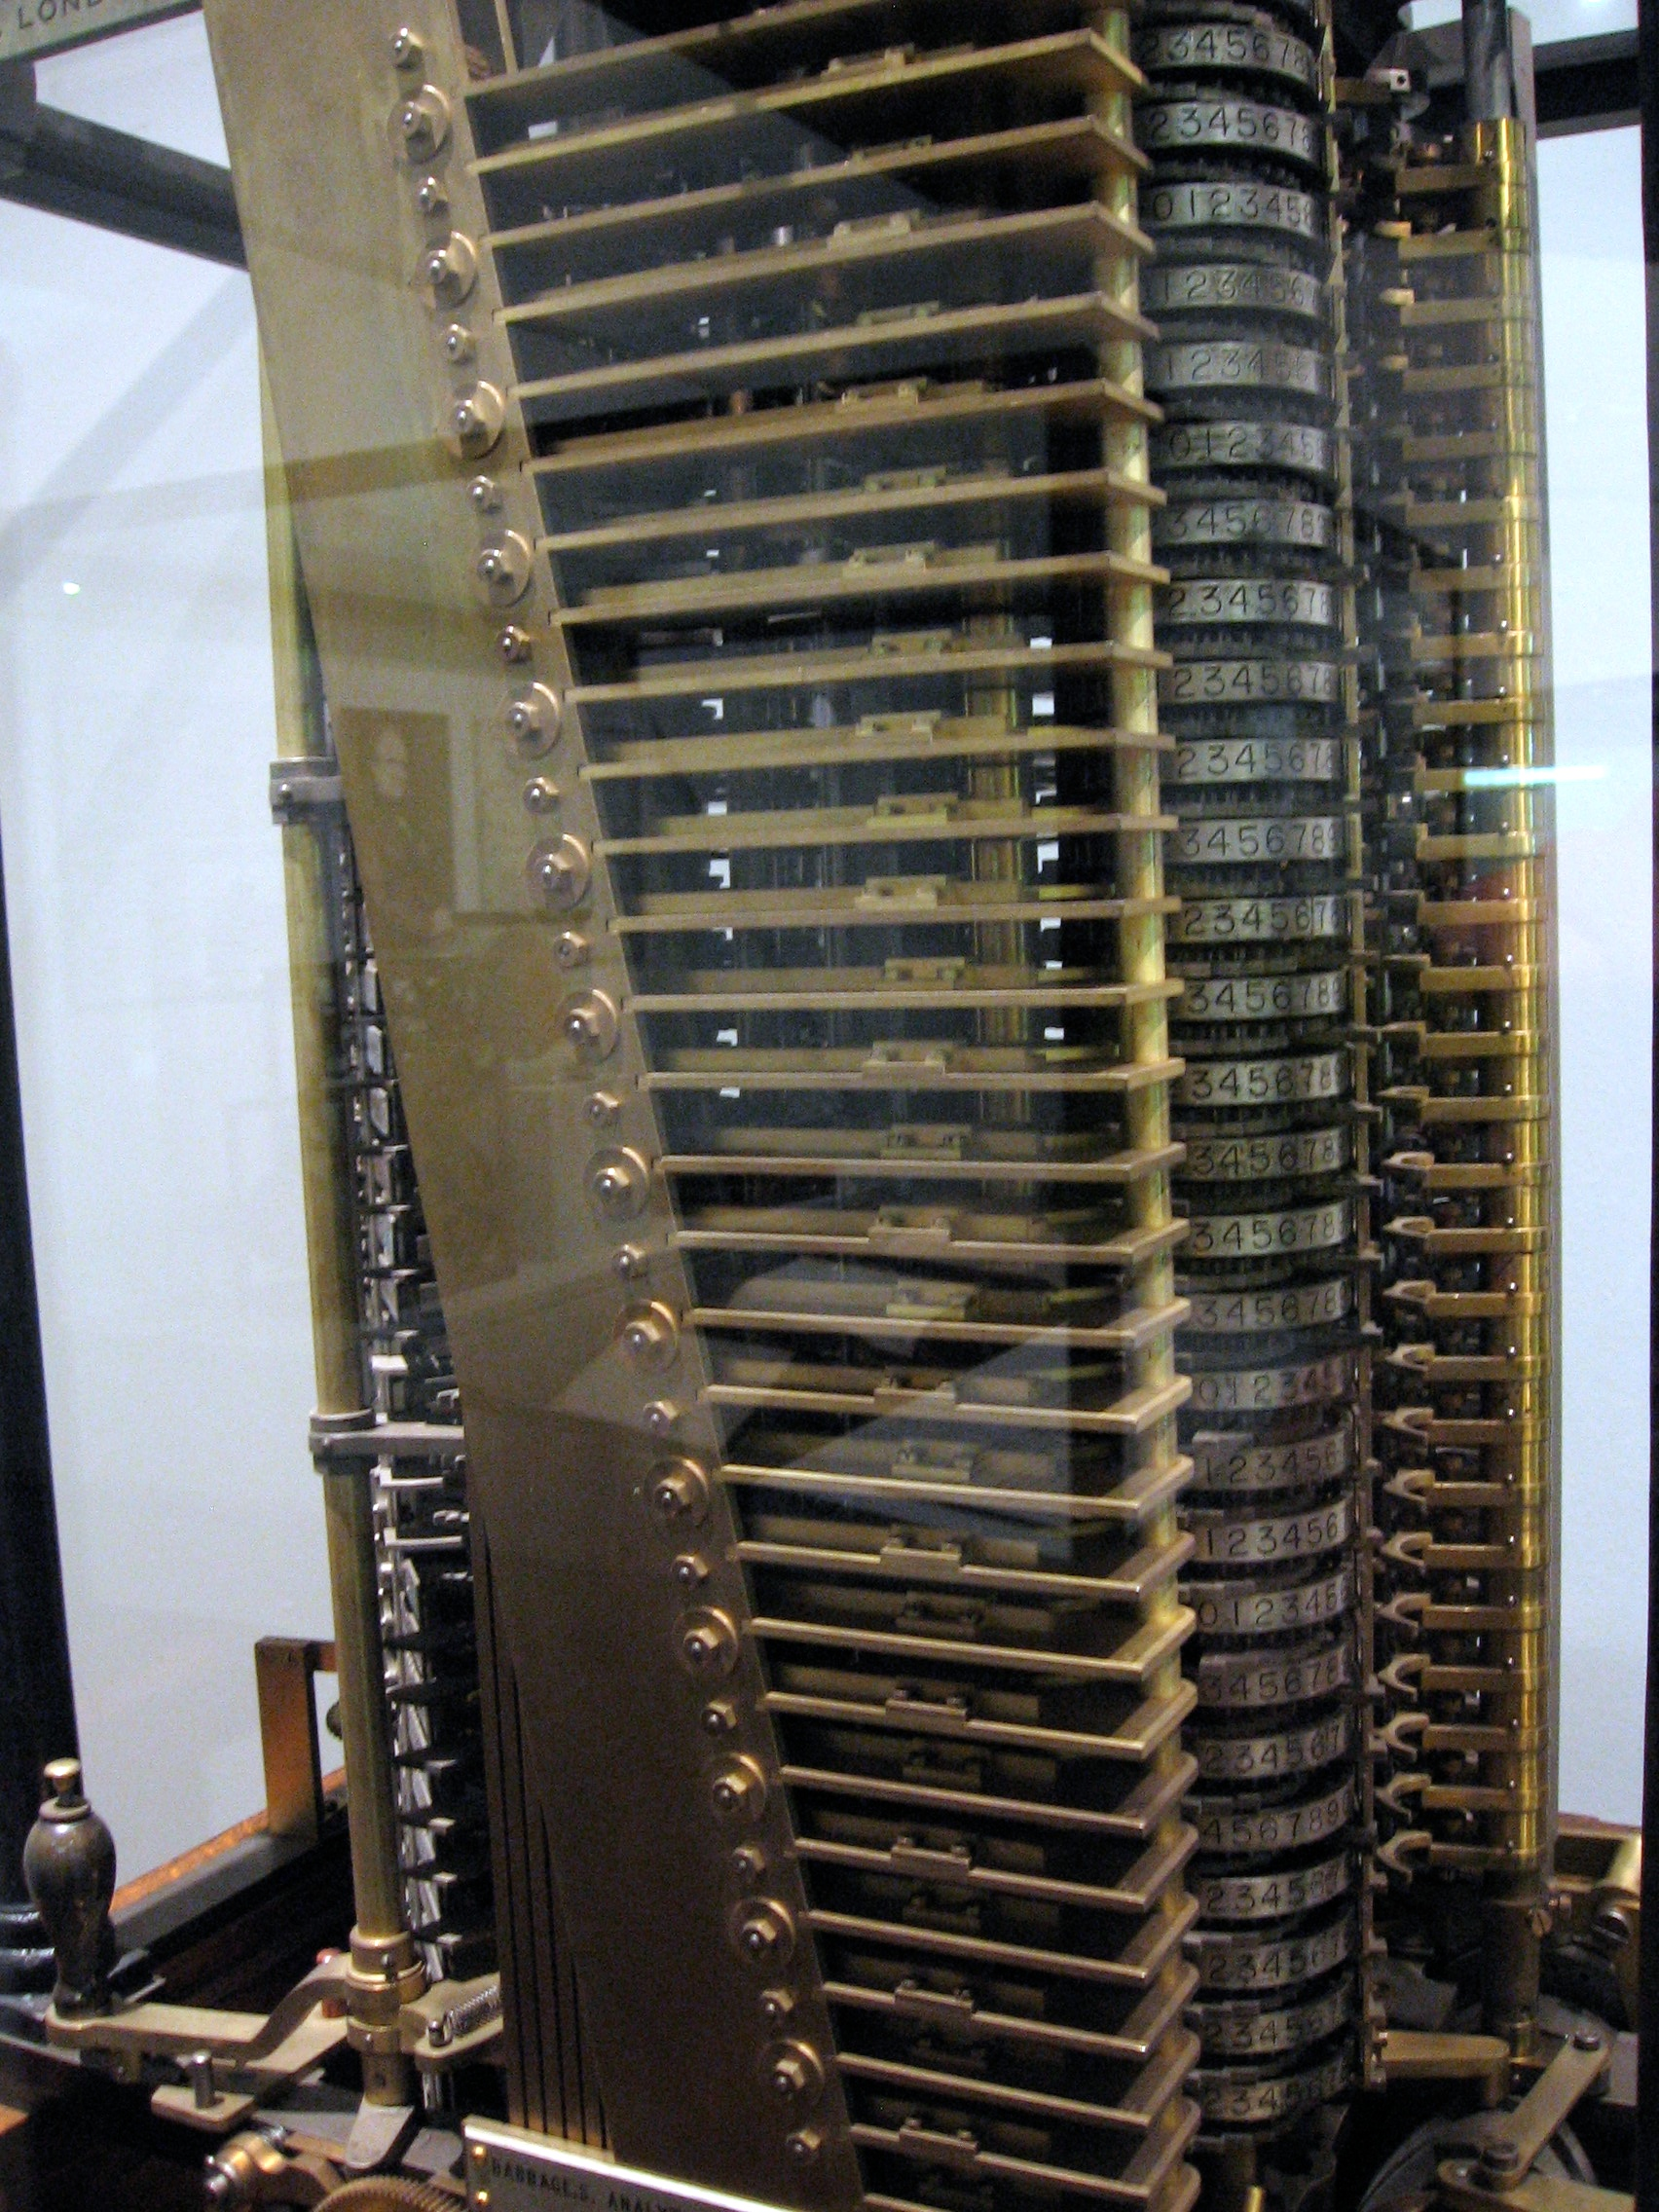
\includegraphics[height=.33\textheight]{images/AnalyticalEngineMill.jpg}\ 
          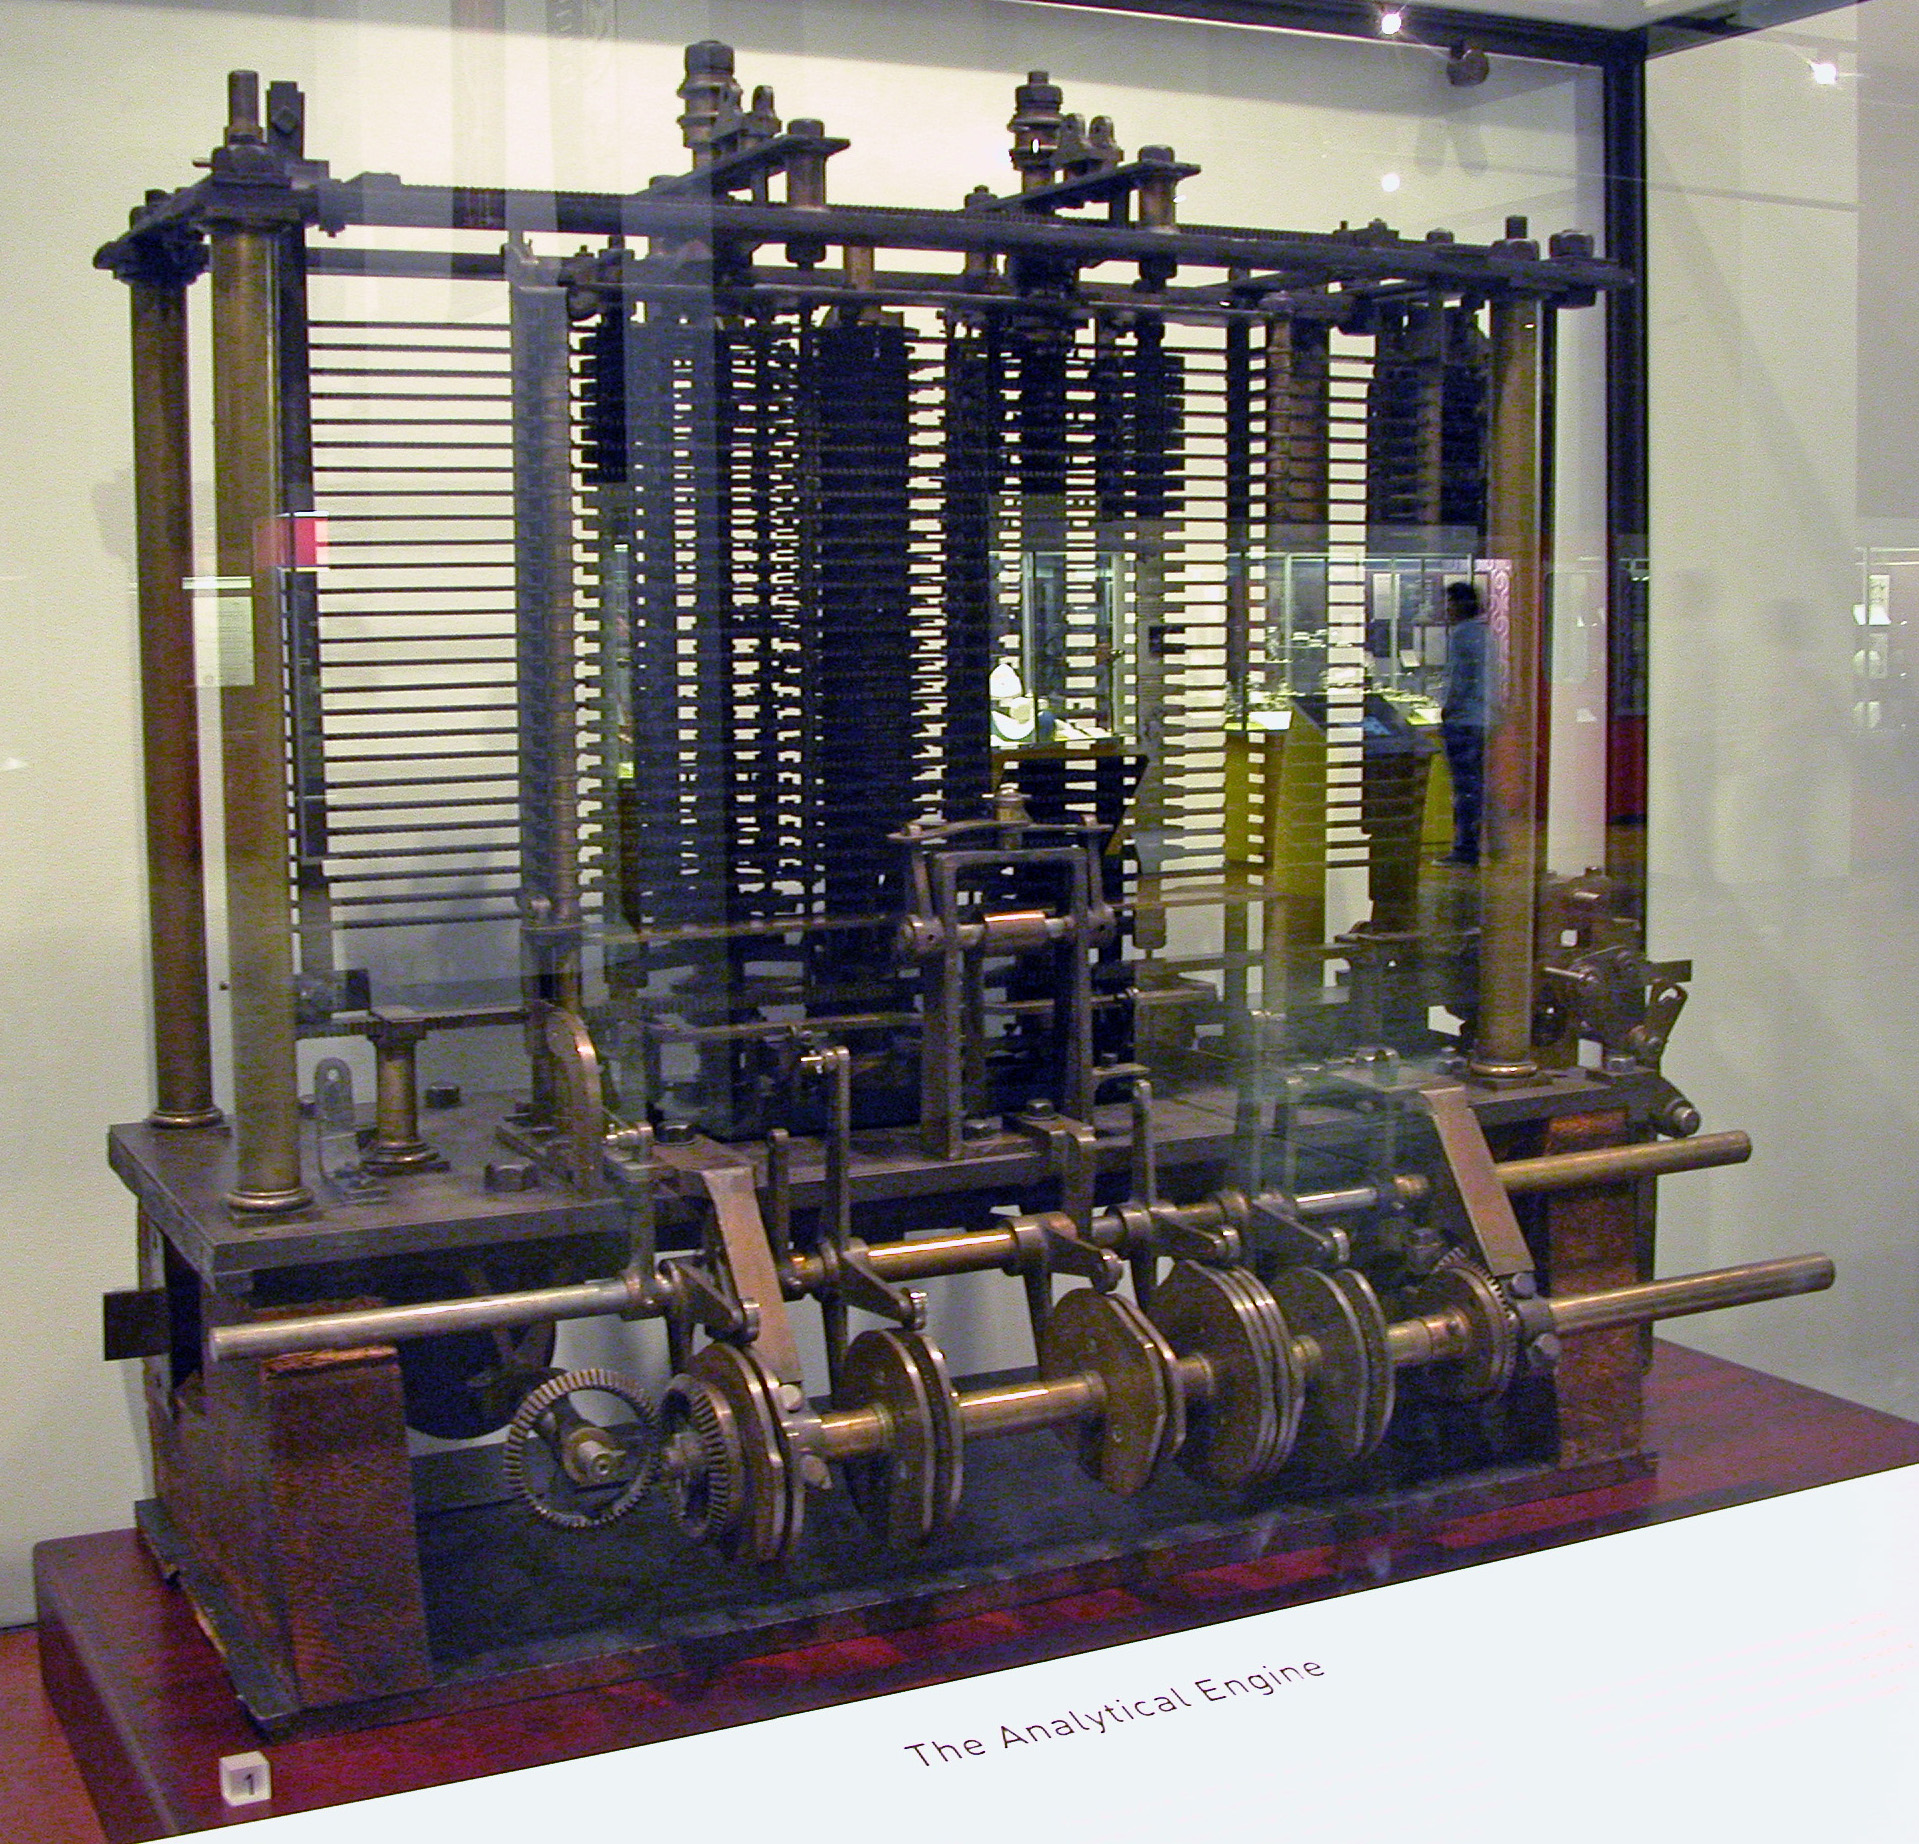
\includegraphics[height=.33\textheight]{images/AnalyticalEngineModel.jpg}\ 
          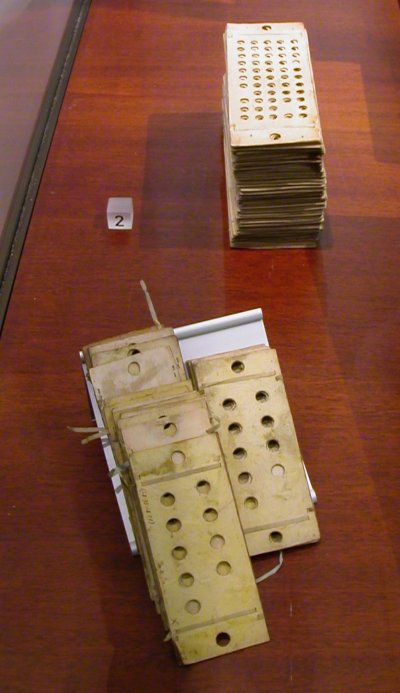
\includegraphics[height=.33\textheight]{images/AnalyticalEnginePunchedCards.jpg}
        \end{center}
      \end{exampleblock}
      \begin{block}{Состав}
        \begin{itemize}
          \item {<<Склад>>}.
          \item {<<Мельница>>}.
          \item Устройство управления.
          \item Устройства ввода и вывода данных.
        \end{itemize}
      \end{block}
    \end{column}
    \begin{column}[]{0.45\textwidth}  
      \begin{block}<1->{Интересные факты}
        \begin{itemize}
          \item {<<Склад>>} в 1000 чисел по 50 десятичных знаков.
          \item Система предварительного (сквозного) переноса при сложении.
          \item Ввод команд для мельницы и склада через  свои перфокарты (отдельные потоки для данных и команд).
          \item Условный переход в обе стороны.
          \item Первая программа: ???
        \end{itemize}
      \end{block}
    \end{column}
  \end{columns}
\end{frame}

%%%%%%%%%%%%%%%%%%%%%%%%%%%%%%%%%%%%%%%%%%%%%%%%%%%%%%%%%%%%%%%%%%%%%%%%%%%%%%%
%%
%% 
%%
\begin{frame}{Архитектура фон Неймана}
  \begin{columns}[T]
    \begin{column}[]{0.45\textwidth}  
      \begin{exampleblock}<1->{Схема}
        \begin{center}
          \begin{tikzpicture}
\node[MyChar, minimum width=3cm, minimum height=1.5cm, text width=2.7cm, align=center] (ALU) at (0,0) {Арифметико-\\логическое\\устройство};
\node[MyChar, minimum width=3cm, minimum height=1.5cm, text width=2.7	cm, align=center] (UU) at (-3.5cm,0) {Управляющее\\устройство};
\node[MyChar, minimum width=6.5cm] (MEM) at (-1.75cm,1.5cm) {Запоминающее устройство};
\node[MyChar, minimum width=6.5cm] (INOUT) at (-1.75cm,-1.5cm) {Устройства ввода/вывода};
\draw[->,double,draw=black!80] (UU) to (UU |- MEM.south);
\draw[->,double,draw=black!80] (UU) to (UU |- INOUT.north);
\draw[<->,double,draw=black!80] (ALU) to (ALU |- MEM.south);
\draw[<->,double,draw=black!80] (ALU) to (ALU |- INOUT.north);
          \end{tikzpicture}
        \end{center}
      \end{exampleblock}
    \end{column}
    \begin{column}[]{0.45\textwidth}  
      \begin{block}<1->{}
        \begin{itemize}
          \item
        \end{itemize}
      \end{block}
    \end{column}
  \end{columns}
\end{frame}

%%%%%%%%%%%%%%%%%%%%%%%%%%%%%%%%%%%%%%%%%%%%%%%%%%%%%%%%%%%%%%%%%%%%%%%%%%%%%%%
%%
%% 
%%
\begin{frame}{}
  \begin{columns}[T]
    \begin{column}[]{0.45\textwidth}  
      \begin{exampleblock}<1->{}
        \begin{center}
        \end{center}
      \end{exampleblock}
    \end{column}
    \begin{column}[]{0.45\textwidth}  
      \begin{block}<1->{}
        \begin{itemize}
          \item
        \end{itemize}
      \end{block}
    \end{column}
  \end{columns}
\end{frame}

\end{document}

